% textidote: ignore begin
\subsection{Classes, Objects and Structure}\label{subsec:classes-objects-and-structure}
% textidote: ignore end

In this section the classes, objects and structure of the proposed solution will be explored, this
will help get a more detail understanding of how the system should function in relation to the problem at hand.


% textidote: ignore begin
\subsubsection{Classes and Objects}\label{subsubsec:classes-and-objects}
% textidote: ignore end
To understand the classes that are relevant for the issues NOVA café is facing,
a general description of the classes is given in Table~\ref{tab:class-table}.

% textidote: ignore begin
\begin{table}[H]
    \centering
    \begin{tabular} { m{2.5cm} m{10cm} }
        \toprule
        \textbf{Classes} & \textbf{Description} \\
        \midrule
        User & The user class is a super class that will keep the
        basic functionality that a user should have.
        Our users are defined as the owners and other staff employed by NOVA café. \\
        \midrule
        Admin & An admin shares most functionality with other user classes,
        but has the highest privileges in the system.
        This means that any admin can create and delete users from the system. \\
        \midrule
        Employee & An employee is a low privilege user class
        that only has access to upload data to the server and
        view the generated statistics and diagrams. \\
        \midrule
        Order & In this context, an order is a customer order,
        that means to buy any of the café's products an order must be created
        for the desired products. \\
        \midrule
        Product & A product is anything that the café sells,
        this could be coffee, food, wine and all other products that
        the café exchanges for money. \\
        \bottomrule
    \end{tabular}
    \caption{A table describing the different classes.}\label{tab:class-table}
\end{table}

\subsubsection{Structure}\label{subsubsec:structure}
% textidote: ignore end

The classes defined in Section~\ref{subsubsec:classes-and-objects} are the building blocks that will be used
to implement the solution.
A way to visualize how the different classes will interact is through a class diagram.
A diagram describing our classes and their interactions can be seen in Figure~\ref{fig:pda-class-diagram}

% textidote: ignore begin
\begin{figure}[H]
    \centering
    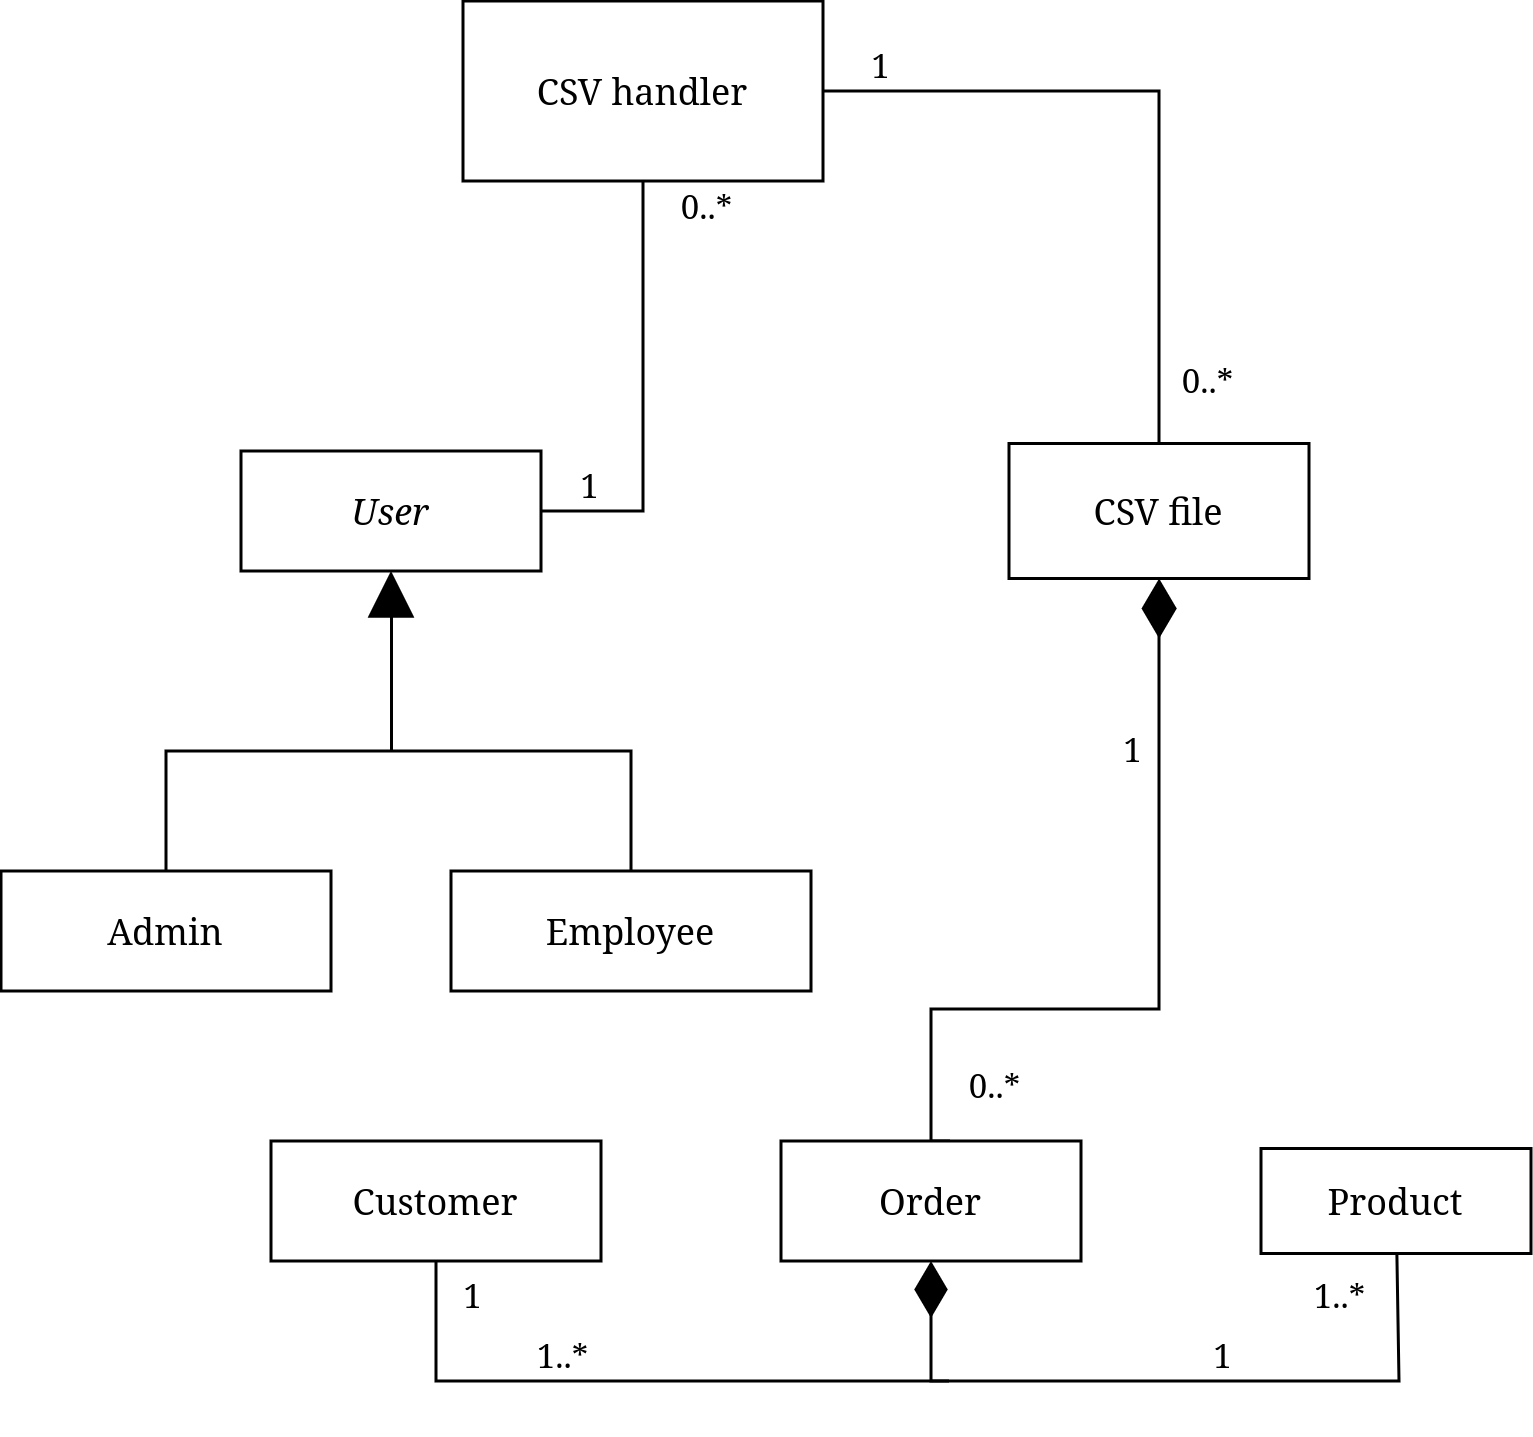
\includegraphics[scale=0.2]{class-overview}
    \caption{Class diagram of the problem domain.}\label{fig:pda-class-diagram}
\end{figure}
% textidote: ignore end
